\section{Results}\label{sec:results}
%Results
%Show effect of colorspaces, blur, annealed mean
%Compare results of architecture (images, error plot, feature maps)

In section \ref{sec:method} all the different techniques and methods used resulted in multiple experiments. This sections shows the different results of each experiment, setting the foundation for the discussion in section \ref{sec:discussion}.

\subsection{Colorspace}
To asses the effect of different colorspaces, a comparison is made between CIELab and YCbCr. The compact network is trained on the landscape set for both the YCbCr and CIELab color space, for a total of 20 epochs. The result is shown in figure \ref{fig:colorspacecomparison}.

\subsubsection{Gaussian blur}
The comparison between different Gaussian blur kernel standard deviations is seen in figure \ref{fig:blur}. The comparison was done with the compact network, trained on the landscape dataset. Note that the standard deviation only comes into play during training, since the target output layer is blurred the target less noisy. It is clear that the case with $\sigma=0$, i.e. no blur, the network was unable to find any colors. Using a blur radius of $\sigma=3$ or $\sigma=5$ leads to much better results. Between these two, the $\sigma=3$ case was chosen to be the best, since it seems more inclined to pick more saturated colors. A too high blur radius will also make the training less effective since the link between texture and color becomes weaker at the edges of objects.

\begin{figure}[h]
	\centering
	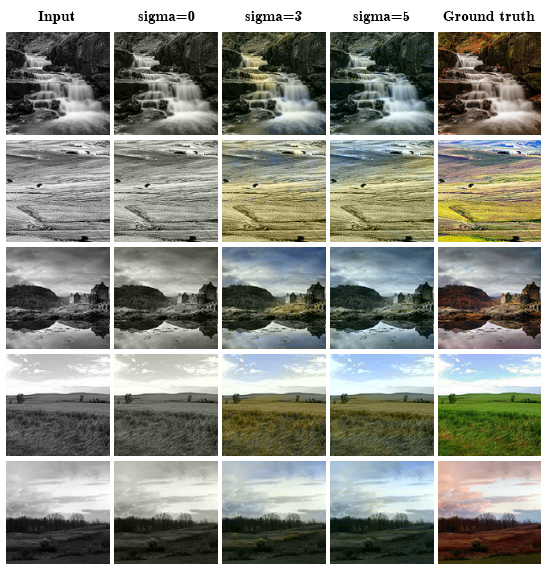
\includegraphics[width=0.6\textwidth]{blur}
	\caption{Blur}
	\label{fig:blur}
\end{figure}

\begin{figure}[h]
	\centering
	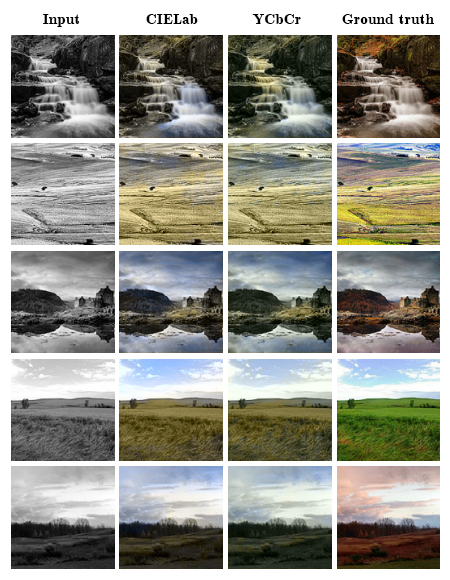
\includegraphics[width=0.6\textwidth]{YCbCr_vs_CIELab}
	\caption{YCbCr vs CIELab}
	\label{fig:YCbCr_vs_CIELab}
\end{figure}

In section \ref{sec:method} all the different techniques and methods used resulted in a selection of five final network architectures with distinct properties. In this section the results of these networks are shown in the form of colorization attempts by the various neural networks.

\begin{figure}[h]
	\centering
	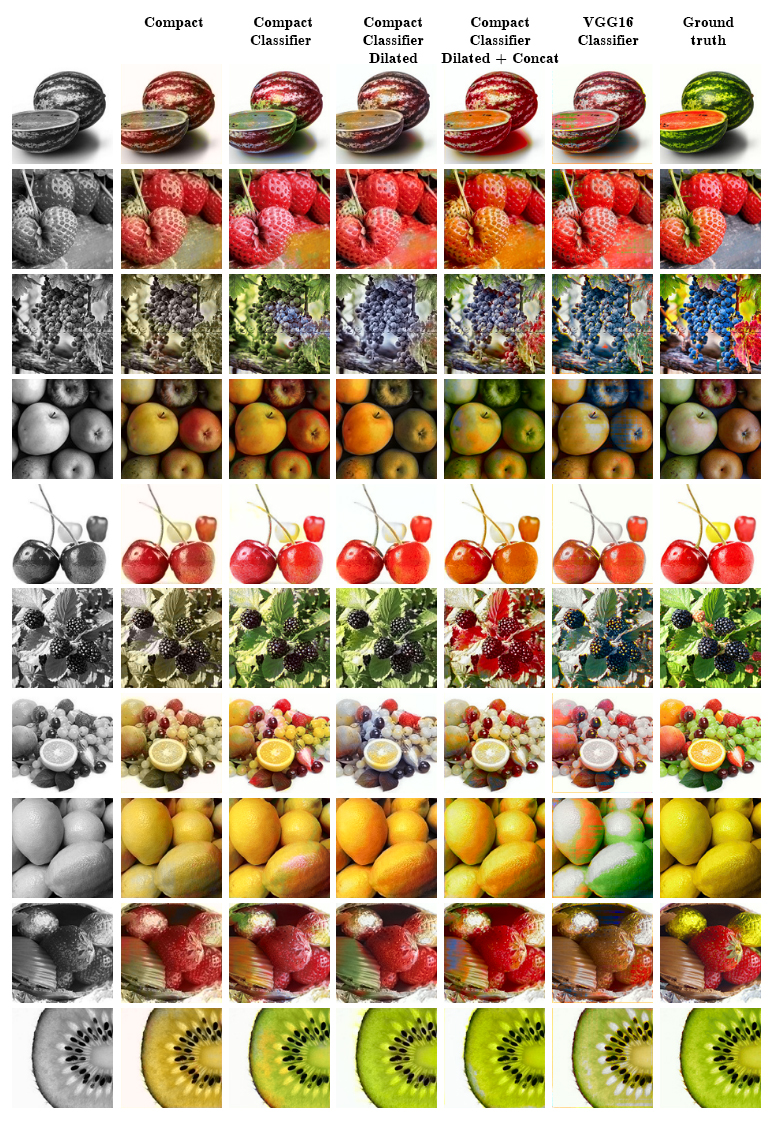
\includegraphics[width=0.9\textwidth]{set1}
	\caption{Results}
	\label{fig:results}
\end{figure}


